\section{High-level languages and tools}
\label{sec:tools}

While ordinary design tools and languages, such as VHDL and Verilog, are not
usually used to synthesize clockless circuits, there is not an
inherent limitation in the languages that prevents this as
demonstrated on \cite[pp. 135-137]{sparso}.

Null convention logic



Most of the work on high-level modeling and synthesis of clockless
circuits is based on the CSP family of languages. The CSP language,
``Communicating Sequential Process'' was proposed by Hoare \cite{csp},
and is based on the mathematical theories of concurrency from process
algebra. CSP-languages allows concurrent processes, composition of
both sequential and parallel statements within a process, and
synchronous message passing between the processes.

\begin{figure}[htbp]
  \centering
  \includegraphics{tangtool.pdf}
  \caption{Tangram design flow. Figure from \cite{fullscan}.}
  \label{fig:tangtool}
\end{figure}

Tangram is a high-level language in the CSP family, designed by
Philips to define clockless circuits. The Tangram compiler generates
what is referred to as handshake circuits, and has its own toolset and
workflow as illustrated in Figure~\ref{fig:tangtool}. Tangram was
later transferred from Philips to the company Handshake Solutions, and
the name of Tangram was changed to Haste. As of this writing, Haste
has entered a state of maintenance, and has been readsorbed into
Philips again.

\begin{figure}[htbp]
  \centering
  \includegraphics{handbuffer.pdf}
  \caption{Handshake buffer a) defined in Balsa source code and b)
    implemented as a handshake circuit. Figure from
    \cite{taylor2008automatic}.}
  \label{fig:handbuffer}
\end{figure}

Handshake circuits, as defined in Tangram, consists of 40 different
basic components that can be connected by four-phase handshake
signalling. The components has active and passive ports, where the
active components initiates the handshake and is said to ``push'' the
data. Figure~\ref{fig:handbuffer}.b illustrates a handshake circuit for
a one-place buffer. Active ports are denoted with a filled circle.

There are multiple circuits implemented in Tangram/Haste. XXX list and
explain different circuits.

Balsa is another CSP-like language based on Tangram, and is an attempt
to define a more expressive language. Balsa also introduces a
intermediate file format, breeze, which contains the netlist for the
handshake components. Breeze can later be implemented into
standard-cell logic by. Figure~\ref{fig:balsatool} shows Balsa and
it's related tools.

Tangram and Balsa are referred to as being a ``syntax-directed''
languages. This means that the silicon compiler transparently and
predictably generates components from each language construct. In
Figure~\ref{fig:handbuffer} it is shown how a simple Balsa-program is
translated into a handshake circuit. Each language-construct, loop,
sequence, transfer, and variable, are translated into handshake
components on a one-to-one basis.

Balsa has for example been used to implement two major circuits: The
DMA-controller for the Amulet3a processor, and the ARM-compatible SPA
processor itself. Balsa is released to the public domain under the
GPLv2 licence.

Handshake component based designs has been shown to use little power,
but also to have low performance \cite{80c51}. Handshake-circuits
exhibit a control heavy structure which inhibits performace. Teak
\cite{teak} introduces a new target component set and synthesis scheme
for synthesizing Balsa circuits as an attempt to mitigate this
drawback. Instead of focusing on control

While Balsa-circuits consists of capacity-less channels, where data on
the channel has to be valid from request to acknowledge, Teak allows
buffers to be automatically inserted into the dataflow, allowing
decoupling. 

Teak circuits have been demonstrated to exhibit 4.6\% to 18.39\% worse
performance than Balsa-circuits when syntehsizing to a fixed gate
delay dual-rail four-phase implementation. However, Teak has a larger
headroom for automated optimising transformations.

\subsection{Testing}

When manufacturing VLSI circuits, it is critical to validate that
units does not contain defects that affect correct functionality. A
common design technique is to ``design for test'', where extra logic
is incorporated into the hardware to facilitate testing. The design
methodology ensures that 

In \cite[pp. 27-28]{sparso} testing is briefly discussed, noting that
the indication-principle will cause a circuit with a stuck-at fault to
deadlock. In \cite[pp. 26]{fullscan}, this is referred to as the
``acknowledge property'', and it is noted that this only holds for the
practical unusefull class of delay-insensitive circuits. In the more
appliciable quasi delay insensitive kind of circuits, generated by
implementing handshake circuits, isochronic forks can extend faults to
not only cause a circuit to deadlock, but also lead to a misbehaving
circuit.

The most common method for running tests on digital circuits is
scan testing. When scan-testing circuits, state-holding elements are
connected into scan-chains that allows the tester to control and
observe the internal (and external) state of the circuit under
test. Industry-standard scan-testing utilises a global-test clock to
steer the testing-procedure. This allows single-stepping the circuit
and by stopping the clock (and traditionally the entire circuit),
$I_{DDQ}$ testing can be performed

Clockless circuits usually uses latches and C-elements for
memory. These memory-elements are not directly scanable, and they are
not connected to any global clock. However, in \cite{fullscan}, it is
shown how Tangram-compiled, clockless, circuits can be made scanable
by replacing all state-holding handshake components with scanable
equivalents. In Figure~\ref{scanC}, from \cite{fullscan}, a scanable
C-element is shown. These components are then connected into a serial
scan chain which is compatible with existing ATPG tools.

It is important to note that the scan-chain insertion is done at the
technology-mapping stage, allowing the designer to insert test-logic
in the final stage of the design-flow.

